% quadsphere.tex -- Quad-Sphere Implementation Notes
% -- Matthew Nicholls

\documentclass[a4paper]{article}
\usepackage{caption}
\usepackage{fontspec}
\usepackage[margin=1in]{geometry}
\usepackage{mathtools}
\usepackage{tikz}

\usetikzlibrary{shapes,shapes.geometric,positioning}

% \setmainfont{Fira Sans}

\begin{document}
  \setlength\parindent{0pt}
  \pagenumbering{gobble}

  \title{Quad-Sphere Implementation Notes}
  \author{Matthew Nicholls}
  \maketitle

  \section*{Vertex Coordinate System}
  A coordinate system for vertices is used to ensure that all quads can retrieve
  the same world position for a given vertex, with the aim to prevent ``seams''
  between quads arising from floating-point imprecision. A vertex coordinate is
  represented as a tuple: $ (\mathit{plane}, a, b) $, where $\mathit{plane}$ is
  the plane of one of the faces of a cube, and $a$ and $b$ are coordinates on that
  plane.

  \begin{figure}[h]
    \centering
  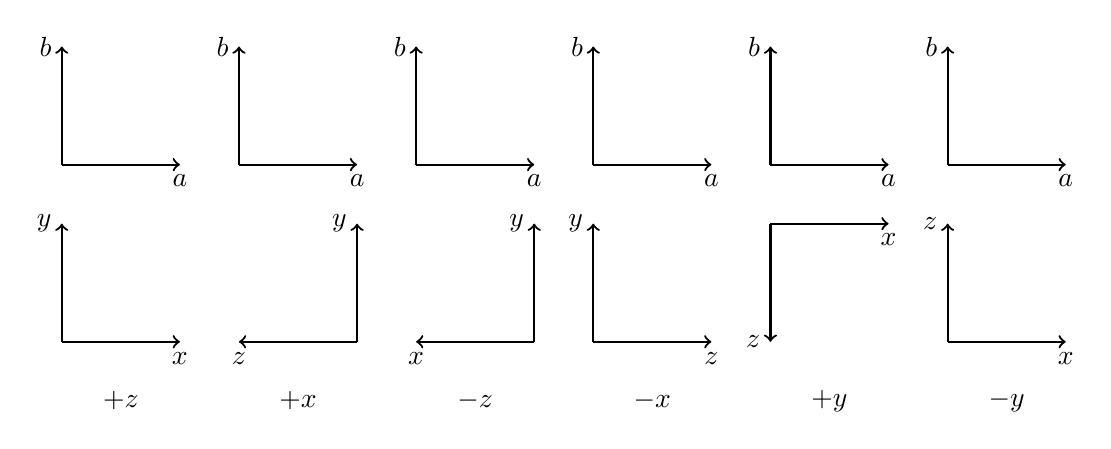
\begin{tikzpicture}[on grid,x=0.75cm,y=0.75cm]
    % ZP
    \node at (1, -1) {$+z$};
    \draw[thick,->] (0, 0) -- (2, 0) node[anchor=north] {$x$};
    \draw[thick,->] (0, 0) -- (0, 2) node[anchor=east] {$y$};

    \draw[thick,->] (0, 3) -- (2, 3) node[anchor=north] {$a$};
    \draw[thick,->] (0, 3) -- (0, 5) node[anchor=east] {$b$};

    % XP
    \node at (4, -1) {$+x$};
    \draw[thick,->] (5, 0) -- (3, 0) node[anchor=north] {$z$};
    \draw[thick,->] (5, 0) -- (5, 2) node[anchor=east] {$y$};

    \draw[thick,->] (3, 3) -- (5, 3) node[anchor=north] {$a$};
    \draw[thick,->] (3, 3) -- (3, 5) node[anchor=east] {$b$};

    % ZN
    \node at (7, -1) {$-z$};
    \draw[thick,->] (8, 0) -- (6, 0) node[anchor=north] {$x$};
    \draw[thick,->] (8, 0) -- (8, 2) node[anchor=east] {$y$};

    \draw[thick,->] (6, 3) -- (8, 3) node[anchor=north] {$a$};
    \draw[thick,->] (6, 3) -- (6, 5) node[anchor=east] {$b$};

    % XN
    \node at (10, -1) {$-x$};
    \draw[thick,->] (9, 0) -- (11, 0) node[anchor=north] {$z$};
    \draw[thick,->] (9, 0) -- (9, 2) node[anchor=east] {$y$};

    \draw[thick,->] (9, 3) -- (11, 3) node[anchor=north] {$a$};
    \draw[thick,->] (9, 3) -- (9, 5) node[anchor=east] {$b$};

    % YP
    \node at (13, -1) {$+y$};
    \draw[thick,->] (12, 2) -- (14, 2) node[anchor=north] {$x$};
    \draw[thick,->] (12, 2) -- (12, 0) node[anchor=east] {$z$};

    \draw[thick,->] (12, 3) -- (14, 3) node[anchor=north] {$a$};
    \draw[thick,->] (12, 3) -- (12, 5) node[anchor=east] {$b$};

    % YN
    \node at (16, -1) {$-y$};
    \draw[thick,->] (15, 0) -- (17, 0) node[anchor=north] {$x$};
    \draw[thick,->] (15, 0) -- (15, 2) node[anchor=east] {$z$};

    \draw[thick,->] (15, 3) -- (17, 3) node[anchor=north] {$a$};
    \draw[thick,->] (15, 3) -- (15, 5) node[anchor=east] {$b$};
  \end{tikzpicture}
  \caption{Shows how the coordinates $(a, b)$ for each plane relate to world coordinates.}
  \end{figure}

  Coordinates $(a, b)$ are integers in the interval $[0,
    C_{max}]$, where $C_{max}$ is calculated as follows:

  \begin{equation}
    C_{max} = 2^{N_{max}} S_q
  \end{equation}
  where $N_{max}$ is the maximum subdivision level and $S_q$ is the size of quad's mesh. 

  \section*{Subdivision}
  \texttt{check\_subdivision} will check what should be done, either:
  \begin{itemize}
    \item Subdivide, if not already, else do nothing.
    \item Collapse, if not already, else do nothing.
    \item Do nothing.
  \end{itemize}
  The test of whether to subdivide or collapse should be mutually exclusive,
  i.e. $ \neg \left(\mathit{Subdivide} \land \mathit{Collapse}\right) $ should
  always be true. This is to prevent the possibility of a quad continuously
  subdividing, then collapsing, then subdividing and so on.

  \section*{Neighbouring Quads}
  An invariant that must be upheld is that no quad should neighbour another quad
  which is more than one subdivision level higher than itself. This is because
  quads only create patching for bridging one subdivision level difference;
  larger differences could theoretically be supported at the cost of additional
  complexity.

  Neighbouring quads are defined as follows: the two quads which also exist in
  the parent quad, e.g. the top left quad has the top right quad to the east,
  and the bottom left to the south; the other two quads are one subdivision
  level lower than the current quad.

  \begin{figure}[h]
    \centering
    \begin{tikzpicture}[on grid,x=0.75cm,y=0.75cm]
      %%\draw (4, 0) -- (8, 0) -- (8, 4) --
      \draw (4, 0) rectangle (8, 4);
      \draw (0, 4) rectangle (4, 8);
      \draw (4, 8) rectangle (8, 12);
      \draw (8, 4) rectangle (12, 8);

      % Subdivided quad
      \draw (4, 6) -- (8, 6);
      \draw (6, 4) -- (6, 8);

      % Centre quad > top left (future) subdivision
      \draw[dashed,dash phase=-1.5pt] (5, 7) -- (4, 7);
      \draw[dashed,dash phase=-1.5pt] (5, 7) -- (6, 7);
      \draw[dashed,dash phase=-1.5pt] (5, 7) -- (5, 6);
      \draw[dashed,dash phase=-1.5pt] (5, 7) -- (5, 8);

      % Centre quad > top right (future) subdivision
      \draw[dashed,dash phase=-1.5pt] (7, 7) -- (6, 7);
      \draw[dashed,dash phase=-1.5pt] (7, 7) -- (8, 7);
      \draw[dashed,dash phase=-1.5pt] (7, 7) -- (7, 6);
      \draw[dashed,dash phase=-1.5pt] (7, 7) -- (7, 8);

      % Centre quad > bottom left (future) subdivision
      \draw[dashed,dash phase=-1.5pt] (5, 5) -- (4, 5);
      \draw[dashed,dash phase=-1.5pt] (5, 5) -- (6, 5);
      \draw[dashed,dash phase=-1.5pt] (5, 5) -- (5, 4);
      \draw[dashed,dash phase=-1.5pt] (5, 5) -- (5, 6);

      % Centre quad > bottom right (future) subdivision
      \draw[dashed,dash phase=-1.5pt] (7, 5) -- (6, 5);
      \draw[dashed,dash phase=-1.5pt] (7, 5) -- (8, 5);
      \draw[dashed,dash phase=-1.5pt] (7, 5) -- (7, 4);
      \draw[dashed,dash phase=-1.5pt] (7, 5) -- (7, 6);

      % Left quad (future) subdivision
      \draw[dashed,dash phase=-1.5pt] (2, 6) -- (0, 6);
      \draw[dashed,dash phase=-1.5pt] (2, 6) -- (4, 6);
      \draw[dashed,dash phase=-1.5pt] (2, 6) -- (2, 4);
      \draw[dashed,dash phase=-1.5pt] (2, 6) -- (2, 8);

      % Right quad (future) subdivision
      \draw[dashed,dash phase=-1.5pt] (10, 6) -- (8, 6);
      \draw[dashed,dash phase=-1.5pt] (10, 6) -- (12, 6);
      \draw[dashed,dash phase=-1.5pt] (10, 6) -- (10, 4);
      \draw[dashed,dash phase=-1.5pt] (10, 6) -- (10, 8);

      % Top quad (future) subdivision
      \draw[dashed,dash phase=-1.5pt] (6, 10) -- (4, 10);
      \draw[dashed,dash phase=-1.5pt] (6, 10) -- (8, 10);
      \draw[dashed,dash phase=-1.5pt] (6, 10) -- (6, 8);
      \draw[dashed,dash phase=-1.5pt] (6, 10) -- (6, 12);

      % Bottom quad (future) subdivision
      \draw[dashed,dash phase=-1.5pt] (6, 2) -- (4, 2);
      \draw[dashed,dash phase=-1.5pt] (6, 2) -- (8, 2);
      \draw[dashed,dash phase=-1.5pt] (6, 2) -- (6, 0);
      \draw[dashed,dash phase=-1.5pt] (6, 2) -- (6, 4);

      \node at (4.5, 5.5) {1};
      \node at (5.5, 5.5) {1};
      \node at (6.5, 5.5) {1};
      \node at (7.5, 5.5) {1};

      \node at (4.5, 6.5) {2};
      \node at (5.5, 6.5) {2};
      \node at (6.5, 6.5) {2};
      \node at (7.5, 6.5) {2};

      \node at (4.5, 7.5) {3};
      \node at (5.5, 7.5) {3};
      \node at (6.5, 7.5) {4};
      \node at (7.5, 7.5) {4};

      \node at (4.5, 4.5) {5};
      \node at (5.5, 4.5) {5};
      \node at (6.5, 4.5) {6};
      \node at (7.5, 4.5) {6};
    \end{tikzpicture}
    \caption{}
    \label{fig:quads}
  \end{figure}
  In Figure \ref{fig:quads}, the numbers group possible ways calculating the second
  type of neighbours described:
  \begin{enumerate}
  \item Our north = our parent's north
  \item Our south = our parent's south
  \item Our north = bottom left quad of our parent's north
  \item Our north = bottom right quad of our parent's north
  \item Our south = top left quad of our parent's south
  \item Our south = top right quad of our parents south
  \end{enumerate}
\end{document}
\endinput
